\documentclass[conference]{IEEEtran}
\IEEEoverridecommandlockouts
% The preceding line is only needed to identify funding in the first footnote. If that is unneeded, please comment it out.
\usepackage{cite}
\usepackage{amsmath,amssymb,amsfonts}
\usepackage{algorithmic}
\usepackage{graphicx}
\usepackage{textcomp}
\usepackage{xcolor}
\usepackage[T1]{fontenc}
\usepackage{newtxtext,newtxmath}
\renewcommand{\bfdefault}{b}
\graphicspath{{./figures}}
\def\BibTeX{{\rm B\kern-.05em{\sc i\kern-.025em b}\kern-.08em
		T\kern-.1667em\lower.7ex\hbox{E}\kern-.125emX}}
\begin{document}
	
	\title{Multi-Floor IPS, a simplified indoor positioning system study*\\
		{\footnotesize \textsuperscript{*}Note: Sub-titles are not captured in Xplore and
			should not be used}
		\thanks{Identify applicable funding agency here. If none, delete this.}
	}
	
	\author{\IEEEauthorblockN{1\textsuperscript{st} Given Name Surname}
		\IEEEauthorblockA{\textit{dept. name of organization (of Aff.)} \\
			\textit{name of organization (of Aff.)}\\
			City, Country \\
			email address or ORCID}
		\and
		\IEEEauthorblockN{2\textsuperscript{nd} Given Name Surname}
		\IEEEauthorblockA{\textit{dept. name of organization (of Aff.)} \\
			\textit{name of organization (of Aff.)}\\
			City, Country \\
			email address or ORCID}
		\and
		\IEEEauthorblockN{3\textsuperscript{rd} Given Name Surname}
		\IEEEauthorblockA{\textit{dept. name of organization (of Aff.)} \\
			\textit{name of organization (of Aff.)}\\
			City, Country \\
			email address or ORCID}
	}
	
	\maketitle
	
	\begin{abstract}
		This document is a model and instructions for \LaTeX.
		This and the IEEEtran.cls file define the components of your paper [title, text, heads, etc.]. *CRITICAL: Do Not Use Symbols, Special Characters, Footnotes, 
		or Math in Paper Title or Abstract.
	\end{abstract}
	
	\begin{IEEEkeywords}
		component, formatting, style, styling, insert
	\end{IEEEkeywords}
	
	\section{Introduction}
	Indoor Positioning Systems (IPS) aim to help users navigate effectively inside of buildings or enclosed areas. This type of navigation proves difficult to create when using common methods for navigation. The most widely used system for navigation is the Global Navigation Satellite System (GNSS) which uses a combination of satellites and ground control stations that aim to calculate ground positions by trilateration. The most well-known GNSS is called the Global Positioning System (GPS). The usage of GPS comes with many caveats as the accuracy of the GPS diminishes when it is used indoors due to the fact that most buildings are built from dense materials like concrete and various metals, which the low power signal from the satellite can not penetrate. The usage of GPS often results in scattering, shadowing, blind spots and signal attenuation, which noticeably affects the accuracy\cite{bgp1}. That is why there have been various methods created for IPS to address the shortcomings of GNSS as well as provide accurate navigation in areas that may not be able to use GNSS
	
	There have been many methods developed for the usage of IPS. One of the most well-known and commonly used methods is trilateration. Trilateration works by measuring signal strength in relation to the distance from the transmitter via Received Signal Strength Indicator (RSSI) fingerprinting \cite{bg2}. The fingerprinting technique consists of two phases. An initial offline phase, and the following online phase. In the offline phase, radio maps are created by collecting RSSI data. The data is then passed onto the online phase where end devices calculate their position based on the coordinates assigned to each RSSI-emitting device, such as Bluetooth Low Energy (BLE) devices. These BLE devices are often used for RSSI fingerprinting due to its low power consumption and ease of deployment. A mobile device can then be used to track a user's location by triangulating the user's device using the distance between the mobile device and the different BLEs. This is a good method as most RSSI signatures are distinct; however, there are shortcomings with this method. An example of a shortcoming is that RSSI is affected by environmental noise, which can cause errors in location estimation\cite{bgp2}. Another shortcoming is that some buildings may be unsuitable for BLEs and BLEs require precision placement to be effective.
	
	The usage of Machine Learning in conjunction with IPS has been shown to be effective to improve the performance of IPS. For example, a work by H.T. Gidey et al. \cite{bgp3} uses online heterogeneous transfer learning to improve the accuracy by combining data from different domains. By using Machine Learning algorithms such as Support vector Machines (SVM), Decision Trees, k-Nearest Neighbor (kNN), Random Forests, and Neural Networks (NN) it may be possible to remedy the shortcomings of IPS systems by treating it as a classification problem. This makes the positioning precision be within a range, so while it may not be able to provide a user's exact location, it can give a relatively reliable estimate on the user's area.
	
	In our previous work, we implemented an IPS using a large grid size (16.75×15m) to reduce the number of classification labels, making the problem more manageable within time constraints. While this approach provided a functional implementation, it left several questions unanswered. Specifically, we sought to determine how the number of data points influences IPS performance, whether a reliable IPS can be implemented with a limited number of BSSID to control feature space complexity, and how small a grid size can be while still maintaining reasonable positioning accuracy.
	Building on this prior work, this paper further explores the use of classification-based IPS by refining our approach to ground truth reliability in experimental settings. We evaluate the effects of feature filtering on model complexity, discuss the trade-offs between grid size and precision, and analyze the advantages and limitations of our implementation. To better quantify accuracy, we introduce two new evaluation metrics: Average Grid from Target (AGT) and Average Distance from Target (ADT). Through this study, we provide deeper insights into the design considerations for IPS, offering practical takeaways for improving indoor positioning accuracy.
	
	
	\section{Literature Review}
	need muic paper here
	
	{\bfseries IndoorGNN}
	In situations where GPS is useless, indoor localization is vital for asset monitoring, security, and navigation. WiFi RSSI-based localization is preferred among various localization technologies because it doesn't require additional infrastructure, given the widespread availability of WiFi access points. However, traditional machine learning methods require large labeled datasets, which are difficult to obtain. This paper introduces IndoorGNN, a Graph Neural Network based model designed to classify indoor locations into predefined regions using WiFi RSSI data. As opposed to conventional methods, IndoorGNN builds a graph representation that dynamically captures spatial interactions at various GNN layers using Dynamic Edge Convolution (DynamicEdgeConv). The model performed better than previous GNN-based methods and traditional ML models (SVM, kNN, and MLP) when tested on the UJIIndoorLoc and MNAV datasets. Additionally, IndoorGNN represents a viable option for real-world applications with limited labeled data since it retains excellent accuracy even with sparse training data.
	
	The experiment results from the UJIIndoorLoc and MNAV datasets are 95.8\% and 97.5\% respectively. Smaller training subsets were used to evaluate the model's robustness, and despite that, it still outperformed other approaches. IndoorGNN is especially useful for asset tracking, emergency management, and indoor navigation in places like malls, hospitals, and warehouses. Future research will focus on conditions where there is more unlabeled data than labeled data, ways to handle missing RSSI values and latitude and longitude determination.  IndoorGNN offers an efficient and precise solution to indoor localisation in a real-world environment where large labeled datasets aren't always available. The source code of IndoorGNN is freely accessible on Github. This paper serves as the primary inspiration for our approach as we use their implementation of IndoorGNN to decide which algorithms to be used to train based on our collected data. 
	
	\textbf{Wayfinding}
	This paper presents the development of an indoor localisation and wayfinding Android application for the University of Edinburgh’s Main Library. The app aims to assist students in navigating the multi-story library by providing real-time location tracking and directions to books, study spaces, and other points of interest. The localization technique is based on Wi-Fi fingerprinting, which estimates the user's position by using the Received Signal Strength Indicator (RSSI) from several access points. After testing several machine learning methods for localization, such as multiple Gaussian Processes, Random Forest, and Nearest Neighbors, single Gaussian Process model produced the best accuracy (1.70 meters RMSE). Navigation is made possible using a topological map produced by the Zhang-Suen thinning algorithm. However, since the layout of the library is difficult navigate, A* search is used to find the shortest path to the intended destination.
	To handle the user's request and interact with the Android app over an API, a Flask-based web server was created. The application scans for Wi-Fi signals, determines the user’s position, and displays a path to the selected destination. Tasks were given to participants to evaluate the accuracy and usability of the system. After completing the tasks, they must also go through a questionnaire, where the feedback was mostly positive. Even though the feedback was positive, there are still problems to be addressed. These problems are limited Wi-Fi scans and Wi-Fi train/test dataset variability. In the future, the system will be expanded to cover more floors, the localization model will be improved, and new app functionality will be included. The results of this experiment show the wider application of Wi-Fi-based indoor navigation systems by being applicable to similar settings such as museums, airports, and hospitals. This paper helps us consider our approach regarding data structure.
	
	\textbf{FootPath}
	This paper presents an infrastructure-free indoor navigation system called FootPath. It provides real-time navigation without GPS, WiFi, or RFID beacons by using sensors on the smartphone, namely the accelerometer and the compass, to determine steps and heading direction. FootPath utilizes OpenStreetMap (OSM) for easy deployment, allowing indoor maps to be added to a global mapping platform. It applies sequence alignment algorithms (inspired by bioinformatics) to match detected steps with expected path in order to improve localisation accuracy and eliminates accumulated drift errors over time. The system has two path-matching methods, First Fit and Best Fit. The former maps detected steps directly onto the expected route and the latter aligns steps dynamically by minimizing mismatches. FootPath provides accurate positioning with an average accuracy of 1.6m for best fit during evaluations in indoor environments. Since it does not require any infrastructure, it is suitable for use in hospitals, museums, trade fairs and historical sites.
	
	With a simple navigation interface that allows users to choose their destination and receive real-time turn-by-turn guidance, FootPath's front end is made with usability in mind. Step detection and heading estimates are used by the system to dynamically update the user's position, showing the current location, estimated route, and next steps. OSM's open-source mapping framework allows crowdsourced map updates, negating the need for proprietary databases for indoor maps. According to evaluations, Best Fit's sequence alignment method is more resistant to sensor errors, which makes it perfect for complex indoor spaces with hallways, elevators, and staircases. Future improvements include being able to track several paths to the same destination to address the issue of the user wandering off. With its open-source mapping, real-time feedback, and sensor-based tracking, FootPath is a scalable and affordable substitute for conventional indoor navigation systems that provides an acceptable option for real-world applications without the need for extra infrastructure. This implementation helps us see how important it is that our implementation is aware of the environment. It also inspired us to look into how to make IPS more simple and compatible with all infrastructure due to their complication within their application. 
	
	\textbf{HAR}
	This paper provides An Overview of Indoor Localization System for Human Activity Recognition (HAR) in Healthcare, especially for the elderly. It looks into how HAR and Indoor Positioning Systems (IPS) may be used to enhance healthcare monitoring. HAR uses wearable sensors, smartphones, or cameras to detect human activities and IPS monitors a person's indoor position. Time of Arrival (TOA), Angle of Arrival (AOA), and Received Signal Strength (RSS) are some of the signal measuring methods highlighted within the study. Each has its benefits and drawbacks. The paper shows how real-time patient tracking, anomaly detection, and emergency help are made possible by smart home and hospital monitoring, which improves healthcare services. Additionally, the paper also looks at how artificial intelligence (AI) and machine learning (ML) may increase the accuracy of HAR and IPS. Deep learning models such as Convolutional Neural Networks (CNNs) improve activity recognition by using sensor data. Hidden Markov Models (HMMs) then help correct positioning errors caused by sensor noise. A privacy-focused method called federated learning is presented, which enables decentralized model training without disclosing private information. Support Vector Machines (SVM), Decision Trees (DT), and Artificial Neural Networks (ANN) are examples of hybrid machine learning algorithms that optimize pattern recognition and tracking effectiveness. The accuracy of activity recognition for senior care in homes and nursing homes is examined in this paper using localization technologies. It examines a range of indoor positioning methods and technologies, evaluating their advantages, disadvantages, and selection standards according to energy efficiency, scalability, accuracy, and cost. The paper emphasizes that while there isn't a one-size-fits-all solution, future IoT and hybrid technologies can improve system performance by combining several localization techniques. As this paper represents many machine learning algorithms, it helps us explore which algorithms are suitable for our collected data.
	
	\textbf{bg3}
	Although WiFi-based positioning is cost-effective, it has poor indoor accuracy due to  signal fluctuations from blocking and reflection. This paper proposes an improved KNN-based fingerprint localization algorithm (P-KNN) that dynamically predicts node positions and filters out reference points (RP) without similar Received Signal Strength (RSS) vectors. This is in contrast to regular KNN and as a result, it reduces computational and time complexity. It also uses historical label position to predict the user’s next position, smoothing out location estimates. This approach improves positioning accuracy and system stability.
	Results from simulation tests of P-KNN against KNN shows that average positioning error is lower, especially in tighter areas. Thus, positioning drift is minimized, and localisation becomes more accurate. A test at one of the college buildings shows an average error reduction from 4.12m to 3.65m in some locations. This research highlights that combining predictive modeling with KNN-based fingerprinting can significantly enhance indoor positioning systems. While this paper acknowledges the use of the P-KNN algorithm, we are not using their full implementation. Instead, we are mainly focusing on evaluating the base model.
	
	\textbf{bg6}
	This paper presents an enhanced RSS fingerprinting-based indoor positioning system using Random Forest (RF) classification. Existing RF-based systems rely only on 2.4 GHz signals, limiting performance due many peripherals and household devices sharing the same frequency. Instead of using only 2.4 GHz signal, the proposed method also uses 5 GHz signal to gain more accuracy. To mitigate the impacts of radio irregularity, RSS measurements are also taken at each reference point (RP) from four different antenna orientations: North, East, South, and West. 
	Experiments were conducted in a lecture room at Yangon Technological University, where 264 reference points (RPs) were defined 0.6m apart. The frequency bands of 2.4 GHz and 5 GHz are both collected from all 4 APs at each RP. The proposed system outperformed existing RF-based indoor positioning approaches. The Random Forest classifier with 400 decision trees produced the highest accuracy, with a positioning error of 1.69 meters. This paper helps us explore Random Forest to evaluate with our collected data. We acknowledge this paper using 2 different Wi-Fi frequencies, however we are not implementing it in our paper.
	
	\section{Methodology}
	This experiment was conducted on the 6th floor and 7th floor hallways of the CMKL building. To match the physical environment to the virtual environment, 1 metre by 1 metre grids were measured, taped and labelled on the floor. The criteria for usable grids were grids that were in the hallway and grids that did not have a permanent obstruction in place like a vending machine or a printer. The total amount of grids per floor was around 600+ grids. After the grids were created, data was collected through the use of two android phones. 
	
	An issue we found when taping the 6th floor was that some areas of the floor had different tilling panels as well as orientation. This caused difficulties as the uniformity of the floor tiles helped provide us with a way to accurately measure the straightness of the 1 metre grid, which was done by measuring the distance of the edge grooves of the tile towards the edge of the 1 metre grid and checking if it provided the same distance. This issue occurred in two areas, the cafeteria area, and the study area.
	
	For the cafeteria area, the issue was easily resolved as we could measure the difference in distance from the groove of the normal tile and the groove of the cafeteria tile, then add or subtract it from the edge measurement. 
	
	
	For the lounge area, it was significantly more difficult to deal with due to the fact that the tiles used were of different sizes as well as different orientation. To handle this we created a single straight line onto the lounge area with a tape measure from a point, then proceeded to take 1 metre measurements of that tape measure to create grids. 
	
	Another problematic thing to note is the fact that the area used for our experiment is subject to wear and tear conditions, as human traffic as well as cleaners cleaning the area can cause some of the tape to be torn apart or moved slightly, which may result in an inaccurate grid.  
	
	This experiment was conducted on the 6th floor and 7th floor hallways of the CMKL building. To match the physical environment to the virtual environment, 1 metre by 1 metre grids were measured, taped and labelled on the floor. The criteria for usable grids were grids that were in the hallway and grids that did not have a permanent obstruction in place like a vending machine or a printer. The total amount of grids per floor was around 600+ grids. After the grids were created, data was collected through the use of two android phones. The mobile application used on the android devices was taken from an open source project of the paper called “ML-BASED MULTI-FLOOR IPS: A COMPARISON”\cite{bgp4}. This mobile application allows us to upload a map of the area and then segment it into identically sized grids.
	
	
	During the taping of the 6th floor, we encountered some challenges related to the varying types and orientations of the tiling panels in certain areas. This created a slight deviation from the uniformity of the floor tiles, which we were relying on to accurately measure the straightness of the 1-meter grid. To measure this, we typically used the distance from the edge grooves of the tiles to the edge of the 1-meter grid, checking for consistency. However, we were able to overcome these challenges in two key areas: the cafeteria and the study area.
	
	In the cafeteria, the solution was straightforward. We simply measured the difference in distance between the grooves of the standard tiles and those used in the cafeteria. By adjusting the measurements accordingly, we were able to maintain an accurate grid despite the variation in tile type.
	
	The lounge area presented a more complex challenge due to the tiles being different sizes and orientations. To address this, we created a single straight line across the lounge using a tape measure from a fixed point. We then took 1-meter measurements along the tape to establish the grid, ensuring accuracy despite the initial tile variations.
	
	Additionally, we had to account for the wear and tear on the area used for our experiment. Human traffic and cleaning activity had the potential to slightly shift or damage the tape, which could impact the grid's accuracy. However, by monitoring and adjusting for any movement in the tape, we were able to maintain the integrity of our measurements throughout the process.
	
	
	The data collected resulted in xxx amount of points collected for floor 7 and xxx amount of points collected for floor 6
	
	
	\section{Result}
	The dataset used in this study consisted of 12,640 data points collected across 1x1m\textsuperscript{2} grids distributed among the floors of our experimental setup. By filtering the available BSSID to utilize only SSID with ‘kmitl’ or ‘cmkl’ we end up with 392 unique BSSID, spanning across the 2 floors of the experiment. A rationale behind filtering WiFi signals in this experiment is to determine whether only easily known BSSID can be utilized in implementing IPS. 9019 data points were collected on 6th floor and 3621 data points were collected on 7th floor.
	
	To explore how different parameter settings impact model training, we systematically iterate through various configurations, training the model multiple times under each setting. The table below highlights the best results observed. Notably, the highest accuracy and the best AGT (Adaptive Generalization Tradeoff) do not come from the same parameter setting. This suggests that these metrics prioritize different aspects of performance—optimizing for accuracy does not necessarily yield the best AGT and vice versa. This insight provides a key perspective as we analyze the results in more detail.
	
	\begin{figure}[htbp]
		\centerline{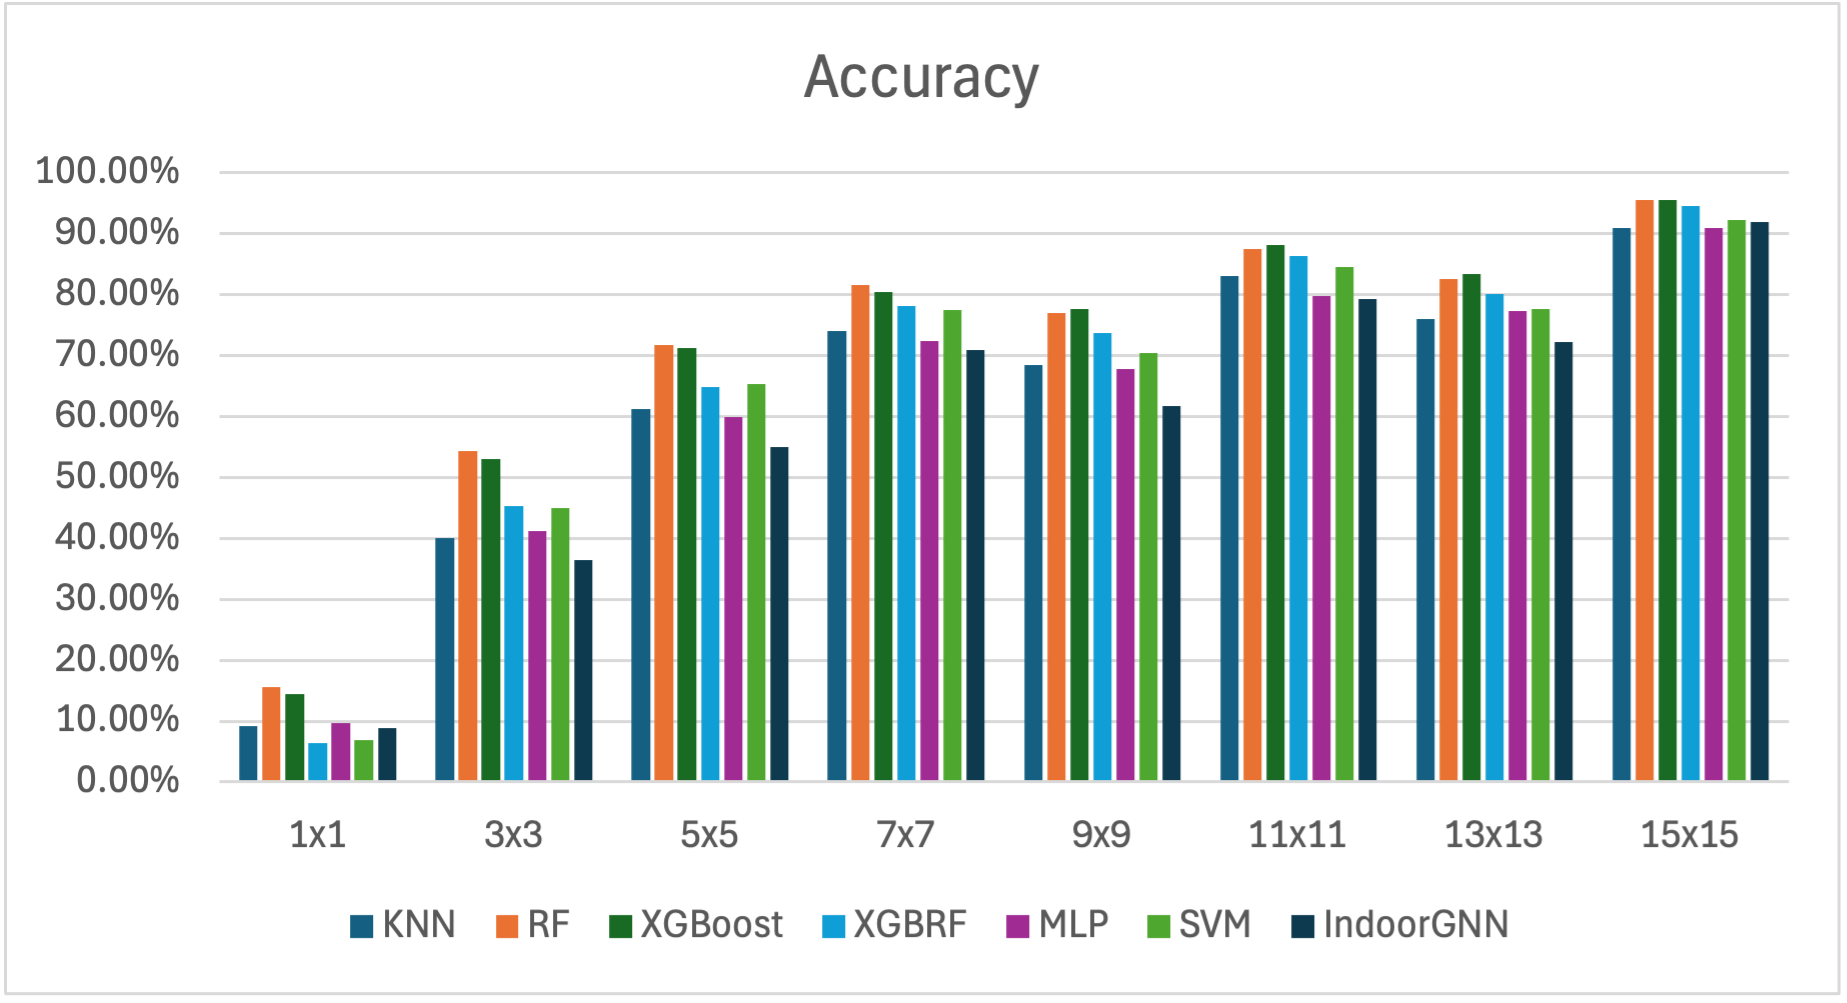
\includegraphics[scale=0.65]{image3.png}}
		\caption{Model Accuracy on Different grid size}
		\label{fig1}
	\end{figure}
	
	\begin{figure}[htbp]
		\centerline{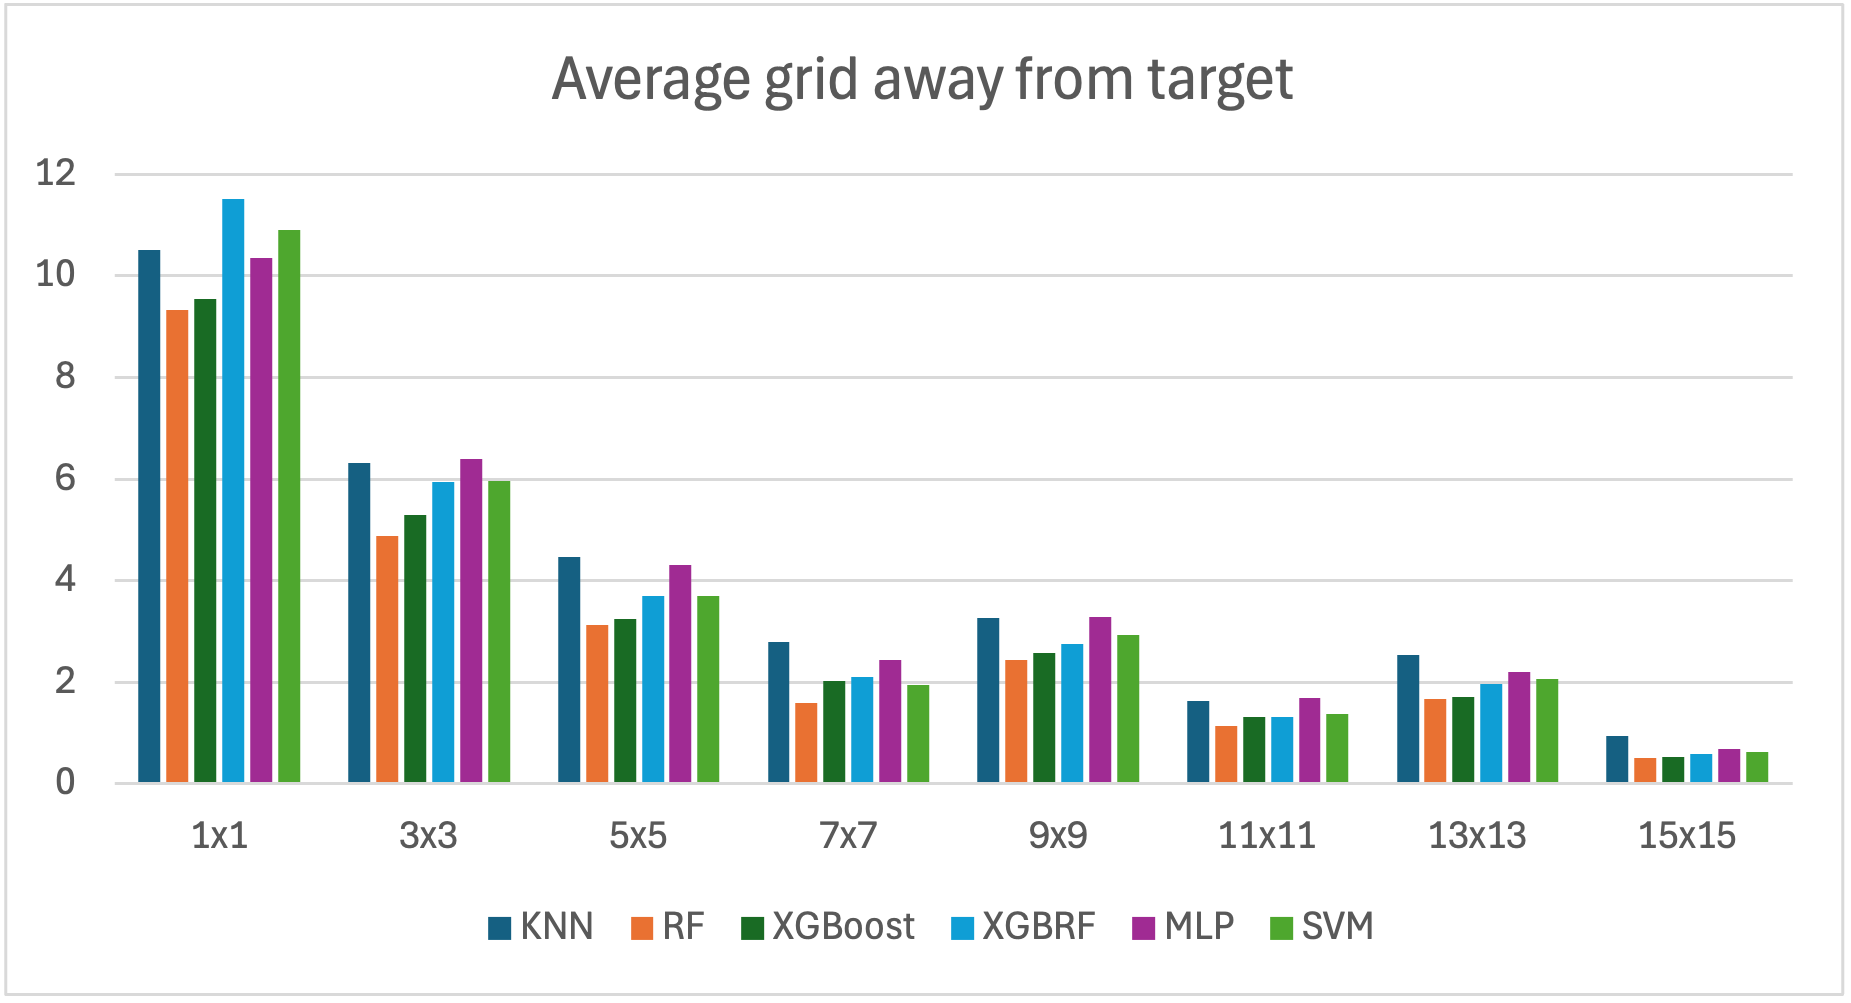
\includegraphics[scale=0.65]{image1.png}}
		\caption{Model Average grid away from Target on Different grid size}
		\label{fig2}
	\end{figure}
	
	To further analyze the spatial distribution of WiFi signals within our test environment, we generated a BSSID heatmap. This visualization helps illustrate how different access points contribute to the overall feature space used in our IPS model. By mapping the signal strength of each detected BSSID across various grid locations, we can better understand signal propagation patterns and identify potential inconsistencies caused by environmental factors such as interference and signal attenuation. The heatmap serves as a diagnostic tool to evaluate the reliability of WiFi-based positioning in our setup. For clarity, readers should ignore the \textbf{ID} and \textbf{Comment} fields in the heatmap, as these are included solely to ensure the data is plotted correctly.
	
	
	\section{Discussion}
	By conducting our experiment across multiple grid sizes, we can visualize the tradeoff between grid size and precision. To quantify this, we calculate the average grid deviation from the target and multiply it by each grid size’s diagonal length, as shown in (insert fig number). This figure illustrates the expected deviation in predictions when a model is trained on a specific grid size, should an error occur.
	
	While a 15×15m grid size performs well on the graph, it inherently limits accuracy to that resolution. In cases where predictions are correct, the location remains constrained within a 15×15m area, which may not be suitable for applications requiring higher precision—such as those needing to pinpoint areas smaller than this grid size.
	
	Through this experiment, we find that a 7×7m grid size offers the best balance between accuracy and precision. It minimizes error while remaining small enough for use in precision-dependent applications. However, it is important to note that these findings may not generalize to all IPS implementations in different environments. The results suggest that increasing grid size does not necessarily improve accuracy; in some cases, performance actually declines, as shown in the chart. This highlights the need for careful consideration when selecting a grid size based on the specific requirements of an IPS deployment.
	
	\begin{figure}[htbp]
		\centerline{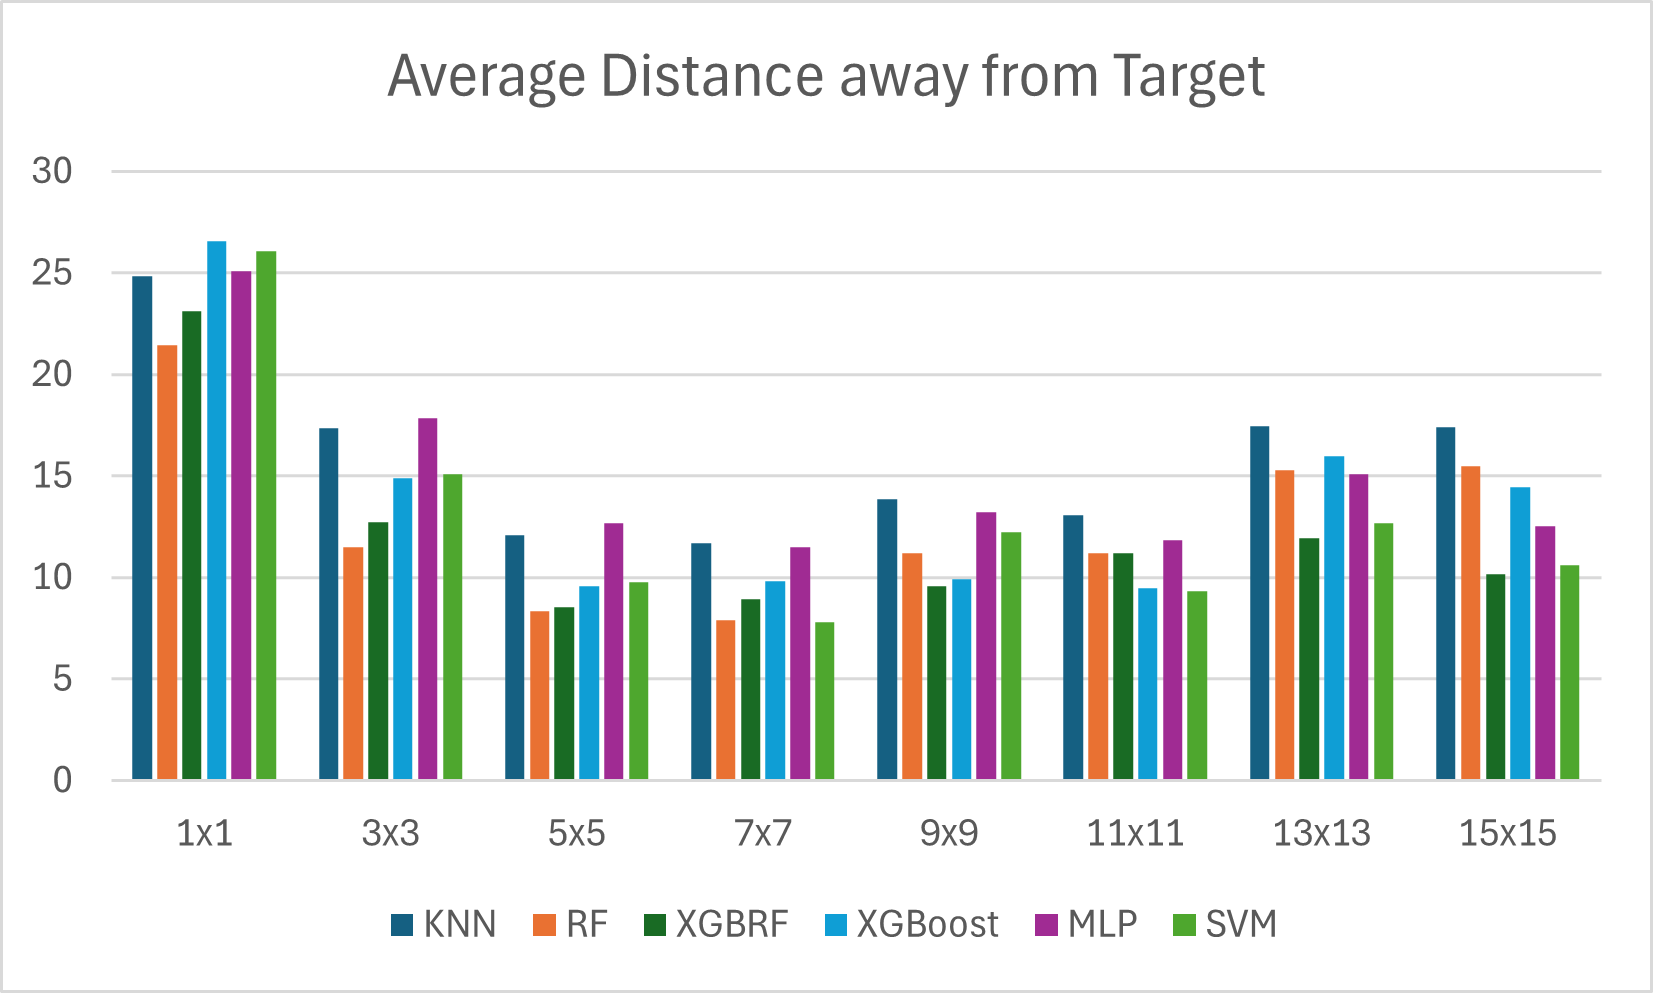
\includegraphics[scale=0.65]{image2.png}}
		\caption{TOBE Caption}
		\label{fig3}
	\end{figure}
	
	Training an IPS model involves significant computational challenges, particularly when dealing with high-dimensional feature spaces. In our experiment, we implemented a simple Wi-Fi access point filtering approach, selecting only access points containing cmkl and kmitl in their names. This drastically reduced the number of access points used as features, making the training process more efficient.
	
	With this filtering method, we were able to train models across multiple grid sizes (1×1, 3×3, 5×5, 7×7, 9×9, 11×11, 13×13, and 15×15) within four days. In contrast, the unfiltered dataset took six days to complete training for just the 1×1 grid size across all target models we intended to test. Due to computational constraints—specifically, the complexity exceeding the capabilities of a single RTX 3080 Ti—we were unable to conduct further experiments with the unfiltered dataset.
	
	Interestingly, our results indicate that filtering access points did not negatively impact the model's learning process. A comparison of training trajectories for the 1×1 grid experiment shows that the filtered model performed comparably to the unfiltered one, if not slightly better in terms of convergence. This suggests that reducing feature dimensionality not only accelerates training but may also make learning more stable.
	
	
	
	\section{Conclusion}
	In conclusion, this paper extends our previous work by refining the implementation of an IPS using a classification-based approach. Through our experiments across multiple grid sizes, we visualized the trade-offs between grid size and precision, showing that increasing grid size does not necessarily improve accuracy and may, in some cases, lead to worse performance. Our findings suggest that a 7×7m grid size offers the best balance between accuracy and precision, making it suitable for applications that require finer localization. However, we acknowledge that these results may not generalize to all environments due to variations in WiFi signal behavior and building structures.
	
	Additionally, we implemented a simple filtering method to limit the number of WiFi BSSID features, preventing excessive model complexity while maintaining comparable performance to an unfiltered approach. This method significantly reduced training time and computational requirements, allowing us to complete model training across multiple grid sizes efficiently. Our results indicate that reducing feature dimensionality not only accelerates training but may also contribute to more stable learning. To better assess IPS performance, we introduced two new evaluation metrics—Average Grid from Target (AGT) and Average Distance from Target (ADT)—which provide a clearer understanding of prediction deviation. Ultimately, our study highlights key considerations in IPS design, particularly in grid size selection and feature filtering, and offers insights for improving indoor positioning accuracy in practical implementations.
	
	
	
	\section{Prepare Your Paper Before Styling}
	Before you begin to format your paper, first write and save the content as a 
	separate text file. Complete all content and organizational editing before 
	formatting. Please note sections \ref{AA}--\ref{SCM} below for more information on 
	proofreading, spelling and grammar.
	
	Keep your text and graphic files separate until after the text has been 
	formatted and styled. Do not number text heads---{\LaTeX} will do that 
	for you.
	
	\subsection{Abbreviations and Acronyms}\label{AA}
	Define abbreviations and acronyms the first time they are used in the text, 
	even after they have been defined in the abstract. Abbreviations such as 
	IEEE, SI, MKS, CGS, ac, dc, and rms do not have to be defined. Do not use 
	abbreviations in the title or heads unless they are unavoidable.
	
	\subsection{Units}
	\begin{itemize}
		\item Use either SI (MKS) or CGS as primary units. (SI units are encouraged.) English units may be used as secondary units (in parentheses). An exception would be the use of English units as identifiers in trade, such as ``3.5-inch disk drive''.
		\item Avoid combining SI and CGS units, such as current in amperes and magnetic field in oersteds. This often leads to confusion because equations do not balance dimensionally. If you must use mixed units, clearly state the units for each quantity that you use in an equation.
		\item Do not mix complete spellings and abbreviations of units: ``Wb/m\textsuperscript{2}'' or ``webers per square meter'', not ``webers/m\textsuperscript{2}''. Spell out units when they appear in text: ``. . . a few henries'', not ``. . . a few H''.
		\item Use a zero before decimal points: ``0.25'', not ``.25''. Use ``cm\textsuperscript{3}'', not ``cc''.)
	\end{itemize}
	
	\subsection{Equations}
	Number equations consecutively. To make your 
	equations more compact, you may use the solidus (~/~), the exp function, or 
	appropriate exponents. Italicize Roman symbols for quantities and variables, 
	but not Greek symbols. Use a long dash rather than a hyphen for a minus 
	sign. Punctuate equations with commas or periods when they are part of a 
	sentence, as in:
	\begin{equation}
		a+b=\gamma\label{eq}
	\end{equation}
	
	Be sure that the 
	symbols in your equation have been defined before or immediately following 
	the equation. Use ``\eqref{eq}'', not ``Eq.~\eqref{eq}'' or ``equation \eqref{eq}'', except at 
	the beginning of a sentence: ``Equation \eqref{eq} is . . .''
	
	\subsection{\LaTeX-Specific Advice}
	
	Please use ``soft'' (e.g., \verb|\eqref{Eq}|) cross references instead
	of ``hard'' references (e.g., \verb|(1)|). That will make it possible
	to combine sections, add equations, or change the order of figures or
	citations without having to go through the file line by line.
	
	Please don't use the \verb|{eqnarray}| equation environment. Use
	\verb|{align}| or \verb|{IEEEeqnarray}| instead. The \verb|{eqnarray}|
	environment leaves unsightly spaces around relation symbols.
	
	Please note that the \verb|{subequations}| environment in {\LaTeX}
	will increment the main equation counter even when there are no
	equation numbers displayed. If you forget that, you might write an
	article in which the equation numbers skip from (17) to (20), causing
	the copy editors to wonder if you've discovered a new method of
	counting.
	
	{\BibTeX} does not work by magic. It doesn't get the bibliographic
	data from thin air but from .bib files. If you use {\BibTeX} to produce a
	bibliography you must send the .bib files. 
	
	{\LaTeX} can't read your mind. If you assign the same label to a
	subsubsection and a table, you might find that Table I has been cross
	referenced as Table IV-B3. 
	
	{\LaTeX} does not have precognitive abilities. If you put a
	\verb|\label| command before the command that updates the counter it's
	supposed to be using, the label will pick up the last counter to be
	cross referenced instead. In particular, a \verb|\label| command
	should not go before the caption of a figure or a table.
	
	Do not use \verb|\nonumber| inside the \verb|{array}| environment. It
	will not stop equation numbers inside \verb|{array}| (there won't be
	any anyway) and it might stop a wanted equation number in the
	surrounding equation.
	
	\subsection{Some Common Mistakes}\label{SCM}
	\begin{itemize}
		\item The word ``data'' is plural, not singular.
		\item The subscript for the permeability of vacuum $\mu_{0}$, and other common scientific constants, is zero with subscript formatting, not a lowercase letter ``o''.
		\item In American English, commas, semicolons, periods, question and exclamation marks are located within quotation marks only when a complete thought or name is cited, such as a title or full quotation. When quotation marks are used, instead of a bold or italic typeface, to highlight a word or phrase, punctuation should appear outside of the quotation marks. A parenthetical phrase or statement at the end of a sentence is punctuated outside of the closing parenthesis (like this). (A parenthetical sentence is punctuated within the parentheses.)
		\item A graph within a graph is an ``inset'', not an ``insert''. The word alternatively is preferred to the word ``alternately'' (unless you really mean something that alternates).
		\item Do not use the word ``essentially'' to mean ``approximately'' or ``effectively''.
		\item In your paper title, if the words ``that uses'' can accurately replace the word ``using'', capitalize the ``u''; if not, keep using lower-cased.
		\item Be aware of the different meanings of the homophones ``affect'' and ``effect'', ``complement'' and ``compliment'', ``discreet'' and ``discrete'', ``principal'' and ``principle''.
		\item Do not confuse ``imply'' and ``infer''.
		\item The prefix ``non'' is not a word; it should be joined to the word it modifies, usually without a hyphen.
		\item There is no period after the ``et'' in the Latin abbreviation ``et al.''.
		\item The abbreviation ``i.e.'' means ``that is'', and the abbreviation ``e.g.'' means ``for example''.
	\end{itemize}
	An excellent style manual for science writers is \cite{b7}.
	
	\subsection{Authors and Affiliations}
	\textbf{The class file is designed for, but not limited to, six authors.} A 
	minimum of one author is required for all conference articles. Author names 
	should be listed starting from left to right and then moving down to the 
	next line. This is the author sequence that will be used in future citations 
	and by indexing services. Names should not be listed in columns nor group by 
	affiliation. Please keep your affiliations as succinct as possible (for 
	example, do not differentiate among departments of the same organization).
	
	\subsection{Identify the Headings}
	Headings, or heads, are organizational devices that guide the reader through 
	your paper. There are two types: component heads and text heads.
	
	Component heads identify the different components of your paper and are not 
	topically subordinate to each other. Examples include Acknowledgments and 
	References and, for these, the correct style to use is ``Heading 5''. Use 
	``figure caption'' for your Figure captions, and ``table head'' for your 
	table title. Run-in heads, such as ``Abstract'', will require you to apply a 
	style (in this case, italic) in addition to the style provided by the drop 
	down menu to differentiate the head from the text.
	
	Text heads organize the topics on a relational, hierarchical basis. For 
	example, the paper title is the primary text head because all subsequent 
	material relates and elaborates on this one topic. If there are two or more 
	sub-topics, the next level head (uppercase Roman numerals) should be used 
	and, conversely, if there are not at least two sub-topics, then no subheads 
	should be introduced.
	
	\subsection{Figures and Tables}
	\paragraph{Positioning Figures and Tables} Place figures and tables at the top and 
	bottom of columns. Avoid placing them in the middle of columns. Large 
	figures and tables may span across both columns. Figure captions should be 
	below the figures; table heads should appear above the tables. Insert 
	figures and tables after they are cited in the text. Use the abbreviation 
	``Fig.~\ref{fig}'', even at the beginning of a sentence.
	
	\begin{table}[htbp]
		\caption{Table Type Styles}
		\begin{center}
			\begin{tabular}{|c|c|c|c|}
				\hline
				\textbf{Table}&\multicolumn{3}{|c|}{\textbf{Table Column Head}} \\
				\cline{2-4} 
				\textbf{Head} & \textbf{\textit{Table column subhead}}& \textbf{\textit{Subhead}}& \textbf{\textit{Subhead}} \\
				\hline
				copy& More table copy$^{\mathrm{a}}$& &  \\
				\hline
				\multicolumn{4}{l}{$^{\mathrm{a}}$Sample of a Table footnote.}
			\end{tabular}
			\label{tab1}
		\end{center}
	\end{table}
	
	\begin{figure}[htbp]
		\centerline{
\includegraphics{fig1.png}}
		\caption{Example of a figure caption.}
		\label{fig}
	\end{figure}
	
	Figure Labels: Use 8 point Times New Roman for Figure labels. Use words 
	rather than symbols or abbreviations when writing Figure axis labels to 
	avoid confusing the reader. As an example, write the quantity 
	``Magnetization'', or ``Magnetization, M'', not just ``M''. If including 
	units in the label, present them within parentheses. Do not label axes only 
	with units. In the example, write ``Magnetization (A/m)'' or ``Magnetization 
	\{A[m(1)]\}'', not just ``A/m''. Do not label axes with a ratio of 
	quantities and units. For example, write ``Temperature (K)'', not 
	``Temperature/K''.
	
	\section*{Acknowledgment}
	
	The preferred spelling of the word ``acknowledgment'' in America is without 
	an ``e'' after the ``g''. Avoid the stilted expression ``one of us (R. B. 
	G.) thanks $\ldots$''. Instead, try ``R. B. G. thanks$\ldots$''. Put sponsor 
	acknowledgments in the unnumbered footnote on the first page.
	
	\section*{References}
	
	Please number citations consecutively within brackets \cite{b1}. The 
	sentence punctuation follows the bracket \cite{b2}. Refer simply to the reference 
	number, as in \cite{b3}---do not use ``Ref. \cite{b3}'' or ``reference \cite{b3}'' except at 
	the beginning of a sentence: ``Reference \cite{b3} was the first $\ldots$''
	
	Number footnotes separately in superscripts. Place the actual footnote at 
	the bottom of the column in which it was cited. Do not put footnotes in the 
	abstract or reference list. Use letters for table footnotes.
	
	Unless there are six authors or more give all authors' names; do not use 
	``et al.''. Papers that have not been published, even if they have been 
	submitted for publication, should be cited as ``unpublished'' \cite{b4}. Papers 
	that have been accepted for publication should be cited as ``in press'' \cite{b5}. 
	Capitalize only the first word in a paper title, except for proper nouns and 
	element symbols.
	
	For papers published in translation journals, please give the English 
	citation first, followed by the original foreign-language citation \cite{b6}.
	
	\begin{thebibliography}{00}
		\bibitem{b1} G. Eason, B. Noble, and I. N. Sneddon, ``On certain integrals of Lipschitz-Hankel type involving products of Bessel functions,'' Phil. Trans. Roy. Soc. London, vol. A247, pp. 529--551, April 1955.
		\bibitem{b2} J. Clerk Maxwell, A Treatise on Electricity and Magnetism, 3rd ed., vol. 2. Oxford: Clarendon, 1892, pp.68--73.
		\bibitem{b3} I. S. Jacobs and C. P. Bean, ``Fine particles, thin films and exchange anisotropy,'' in Magnetism, vol. III, G. T. Rado and H. Suhl, Eds. New York: Academic, 1963, pp. 271--350.
		\bibitem{b4} K. Elissa, ``Title of paper if known,'' unpublished.
		\bibitem{b5} R. Nicole, ``Title of paper with only first word capitalized,'' J. Name Stand. Abbrev., in press.
		\bibitem{b6} Y. Yorozu, M. Hirano, K. Oka, and Y. Tagawa, ``Electron spectroscopy studies on magneto-optical media and plastic substrate interface,'' IEEE Transl. J. Magn. Japan, vol. 2, pp. 740--741, August 1987 [Digests 9th Annual Conf. Magnetics Japan, p. 301, 1982].
		\bibitem{b7} M. Young, The Technical Writer's Handbook. Mill Valley, CA: University Science, 1989.
	\end{thebibliography}
	\vspace{12pt}
	\color{red}
	IEEE conference templates contain guidance text for composing and formatting conference papers. Please ensure that all template text is removed from your conference paper prior to submission to the conference. Failure to remove the template text from your paper may result in your paper not being published.
	
\end{document}
